We perform a systematic study of a class of mobile sensor\footnote{As will be explained, ``mobile sensor'' is used here in a broad sense.} deployment optimization problems targeting the coverage of 2D surfaces embedded in 3D domains, applicable to a broad set of practical settings, for example: (1) the selection of surveillance camera locations for maximizing the joint coverage of an art museum, (2) the deployment of mobile robots with range-based sensing apparatus for the monitoring of complex 3D terrains with quality assurances, and (3) the optimization of UVC light source locations for disinfecting interior surfaces of public indoor spaces, e.g., airplanes, buses, hospital rooms, and schools (Fig.~\ref{fig:ex}), which is of key relevance to the ongoing COVID-19 pandemic. Despite the problems' apparent differences, the above-mentioned tasks fall under the general problem of placing mobile sensors for optimizing some form of coverage. This work is devoted to providing such a unifying problem formulation, understanding its rich structural properties, and delivering effective computational methods for readily solving the multiple variations, which all have high application potentials.

\begin{figure}[!ht]
    \centering
    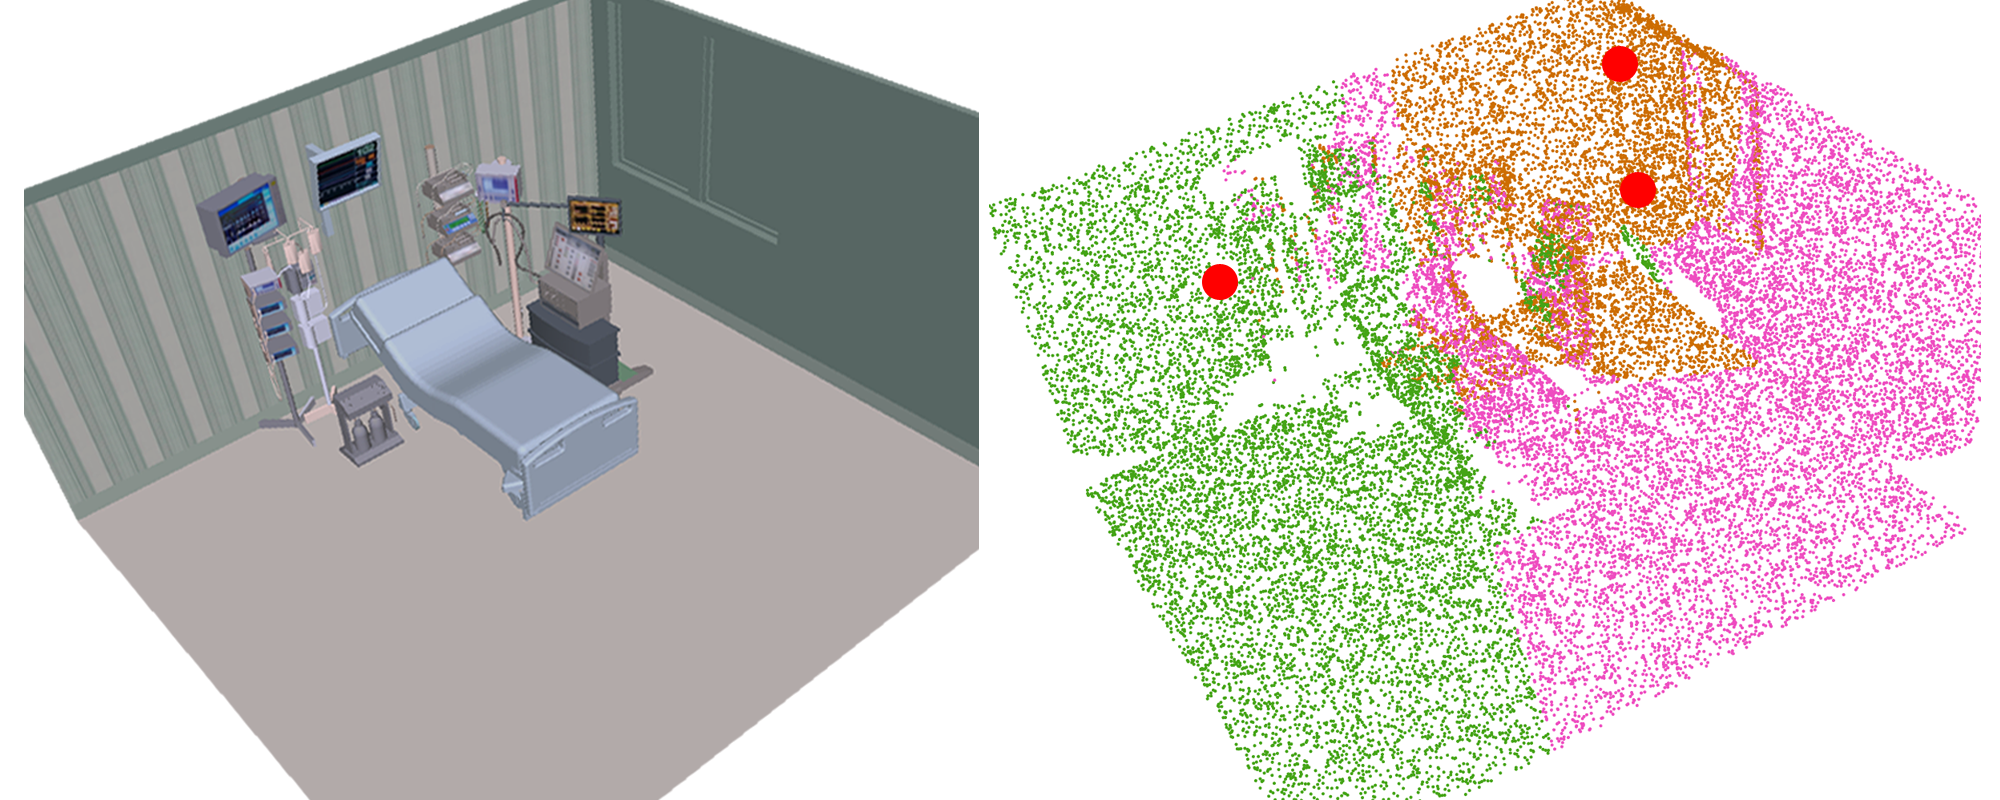
\includegraphics[width=0.95\columnwidth]{chapters/surf/fig/icu-expo.png}
    \vspace{1mm}
    %\hspace{-0.505\columnwidth}
    %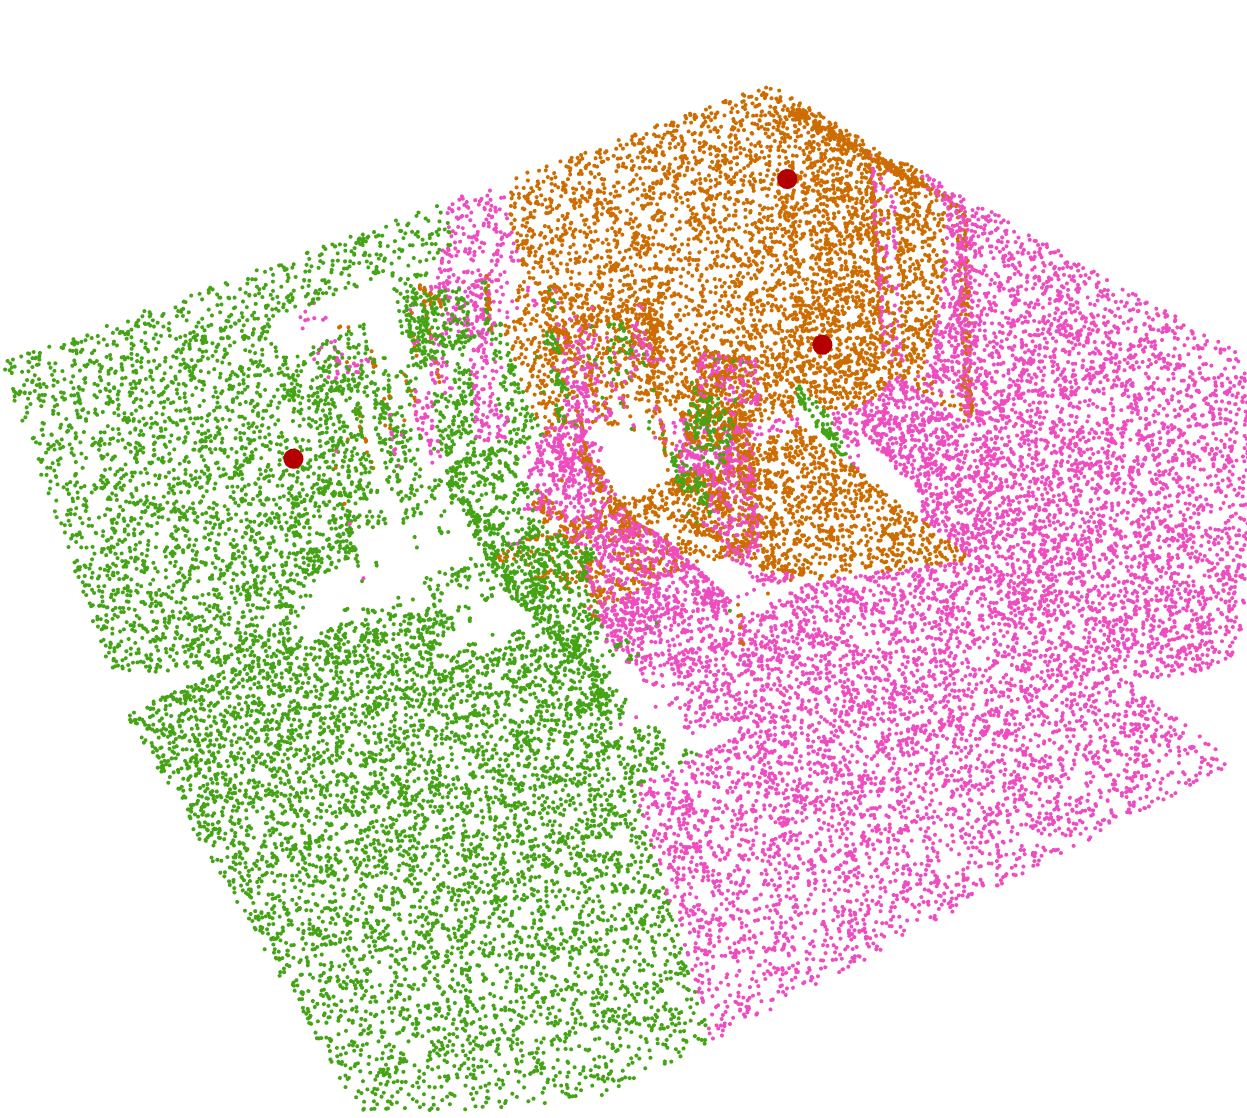
\includegraphics[width=.48\columnwidth]{fig/icu_result_problem3_3.png}
    \caption{[left] The 3D model of an intensive care unit (ICU) in a hospital. [right] A near-optimal coverage of the ICU using three UVC light sources deployed on the ceiling of the room (shown as red discs) where a minimum level of exposure dose can be guaranteed. Each color (orange, green, pink) marks the covered surface locations of a given UVC source. Areas with insufficient exposure are also readily shown as scattered white regions, which can be eliminated through adding more UVC sources.}
    \label{fig:ex}
\end{figure}

As a summary of the research and its contributions, under a general formulation, three coverage optimization problems are examined that are based on \emph{visibility}, \emph{best quality}, and \emph{cumulative quality}, respectively. The visibility model only takes into account line-of-sight sensing. In the best quality model, the coverage quality of a point in the environment is determined by the closest visible sensor, i.e., the quality is determined by distance. A max-min optimization over this quantity is performed. In the cumulative quality model, the coverage of a point is the sum of coverage by all visible ``sensors''. For this model, the area over which a minimum quality can be guaranteed is maximized. Even in simpler 2D settings, these formulations, are known to induce significant computational challenges. They are frequently NP-hard and sometimes hard to approximate, which we briefly discuss. On the algorithmic side, we show how some of these problems can be approximately solved in polynomial time and then develop general integer programming methods, assisted with local improvements, for quickly computing high quality (i.e., $(1+\varepsilon)$-optimal) solutions. Extensive evaluations are performed over multiple realistic application scenarios, confirming the effectiveness of our algorithmic solutions. 

The general formulation and specific models investigated in this work have their origins in two main lines of research: Art Gallery \cite{o1987art,shermer1992recent,o2017visibility} and studies on mobile sensor networks, e.g., \cite{howard2002mobile,cortes2004coverage,martinez2007motion,krause2008near,schwager2009decentralized,hollinger2013sampling}. Our visibility-based model has deep roots in Art Gallery problems \cite{o1987art,shermer1992recent,o2017visibility}, which commonly assume a sensor model based on line-of-sight visibility\cite{lozano1979algorithm}; a main task is to guard every point in the interior of a bounded 2D regions (a point is guarded when it is visible to at least one of the guards). Depending on the exact formulation, guards may be placed on boundaries, corners, or the interior of the region. Not surprisingly, Art Gallery problems are typically NP-hard \cite{lee1986computational}. Other than Art Gallery, 2D coverage problems with other sensing models, e.g., disc-based, have also been considered \cite{thue1910dichteste,hales2005proof,drezner1995facility,cortes2004coverage,pavone2009equitable,pierson2017adapting}. Some formulations prevent the overlapping of individual sensing ranges \cite{thue1910dichteste,hales2005proof} while others seek to ensure a full coverage which often require overlapping sensor coverage.

In an influential body of work \cite{cortes2004coverage,martinez2007motion}, a gradient-based iterative method was devised that drives multiple mobile sensors to a locally optimal coverage configuration, with 
convergence guarantees. 
%
Whereas \cite{cortes2004coverage,martinez2007motion} assume availability of gradients {\em a priori}, such information can also be learned \cite{schwager2009decentralized}. 
%
Subsequently, the method is further extended to allow the coverage of non-convex and disjoint 2D domains \cite{schwager2009optimal} and to work for mobile robots with heterogeneous capabilities \cite{pierson2017adapting}. 
%
In contrast to these iterative local interaction-based methods, this work emphasizes the direct computation of globally optimal solutions under challenging 3D settings. 

 Distributed sensor coverage \cite{cortes2004coverage,schwager2009decentralized} builds on the study of facility location problems \cite{weber1929theory,drezner1995facility} examining the selection of facility (e.g., warehouses) locations that minimize the cost of delivery of goods to spatially distributed customers. These are known (e.g., in operations research and computer science) as clustering problems \cite{har2011geometric}, with many variations depending on the cost structure. Our investigation benefits from the vast literature on clustering and related problems, e.g., \cite{feder1988optimal,hochbaum1985best,gonzalez1985clustering,daskin2000new,shamos1975closest}.
%
Clustering problems are in turn related to packing \cite{hales2005proof}, tiling \cite{thue1910dichteste}, and Art Gallery problems \cite{o1987art,shermer1992recent}.

This work is a continuation of our systematic effort \cite{FenHanGaoYuRSS19,FenYu2020RAL,FenYuRSS20} at tackling sensor coverage problems. Our earlier studies focus on 1D/2D sensors models covering 1D/2D domains, which are significantly less complicated than the 3D settings examined in the current study.

The rest of the paper is organized as follows. In Section~\ref{sec:preliminary}, we provide an umbrella problem statement and detail the three coverage models. Computational complexity of the formulations is briefly discussed. In Section~\ref{sec:algorithm}, we describe effective algorithmic solutions for solving these sensor coverage problems. Extensive evaluation results are provided in Section~\ref{sec:evaluation} containing multiple realistic application settings. We conclude the work in Section~\ref{sec:conclusion}.